\chapter{Implémentation}

\section{Architecture physique et interfaces}

Grâce à l'architecture physique (cf figure \ref{fig:archiPhysique}), nous avons pu déduire que notre projet se décomposait en trois sous-systèmes : les interfaces d'acquisition, logicielle et graphique.

\begin{figure}[H]
  \centering
  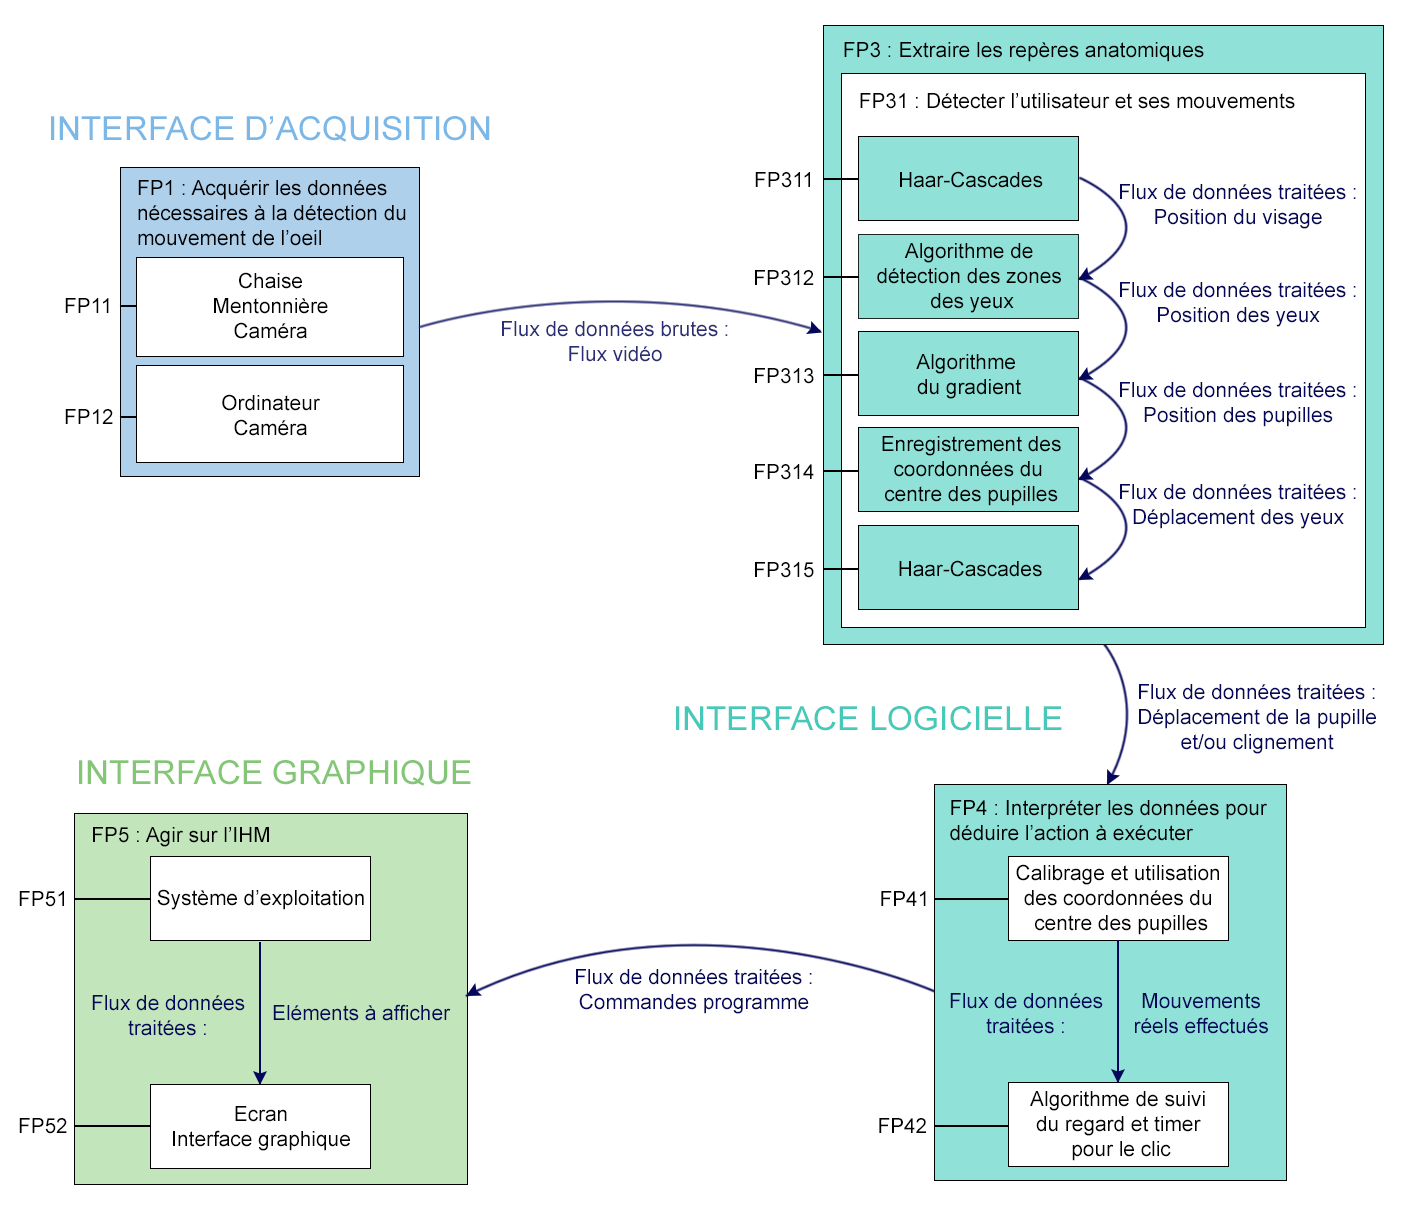
\includegraphics[scale=1.2]{architecturePhysique}
  \caption{Architecture Physique}
  \label{fig:archiPhysique}
\end{figure}

\subsection{Interface d'acquisition}
Cette interface est constituée principalement de la caméra et de la mentonnière (cf figure \ref{fig:systeme}). Cette dernière est utilisée pour éviter les mouvements de la tête, non traités par le programme. L'ordinateur occupe également une place secondaire, puisqu'il permet de vérifier que l'utilisateur est convenablement installé.

\begin{figure}[H]
  \centering
  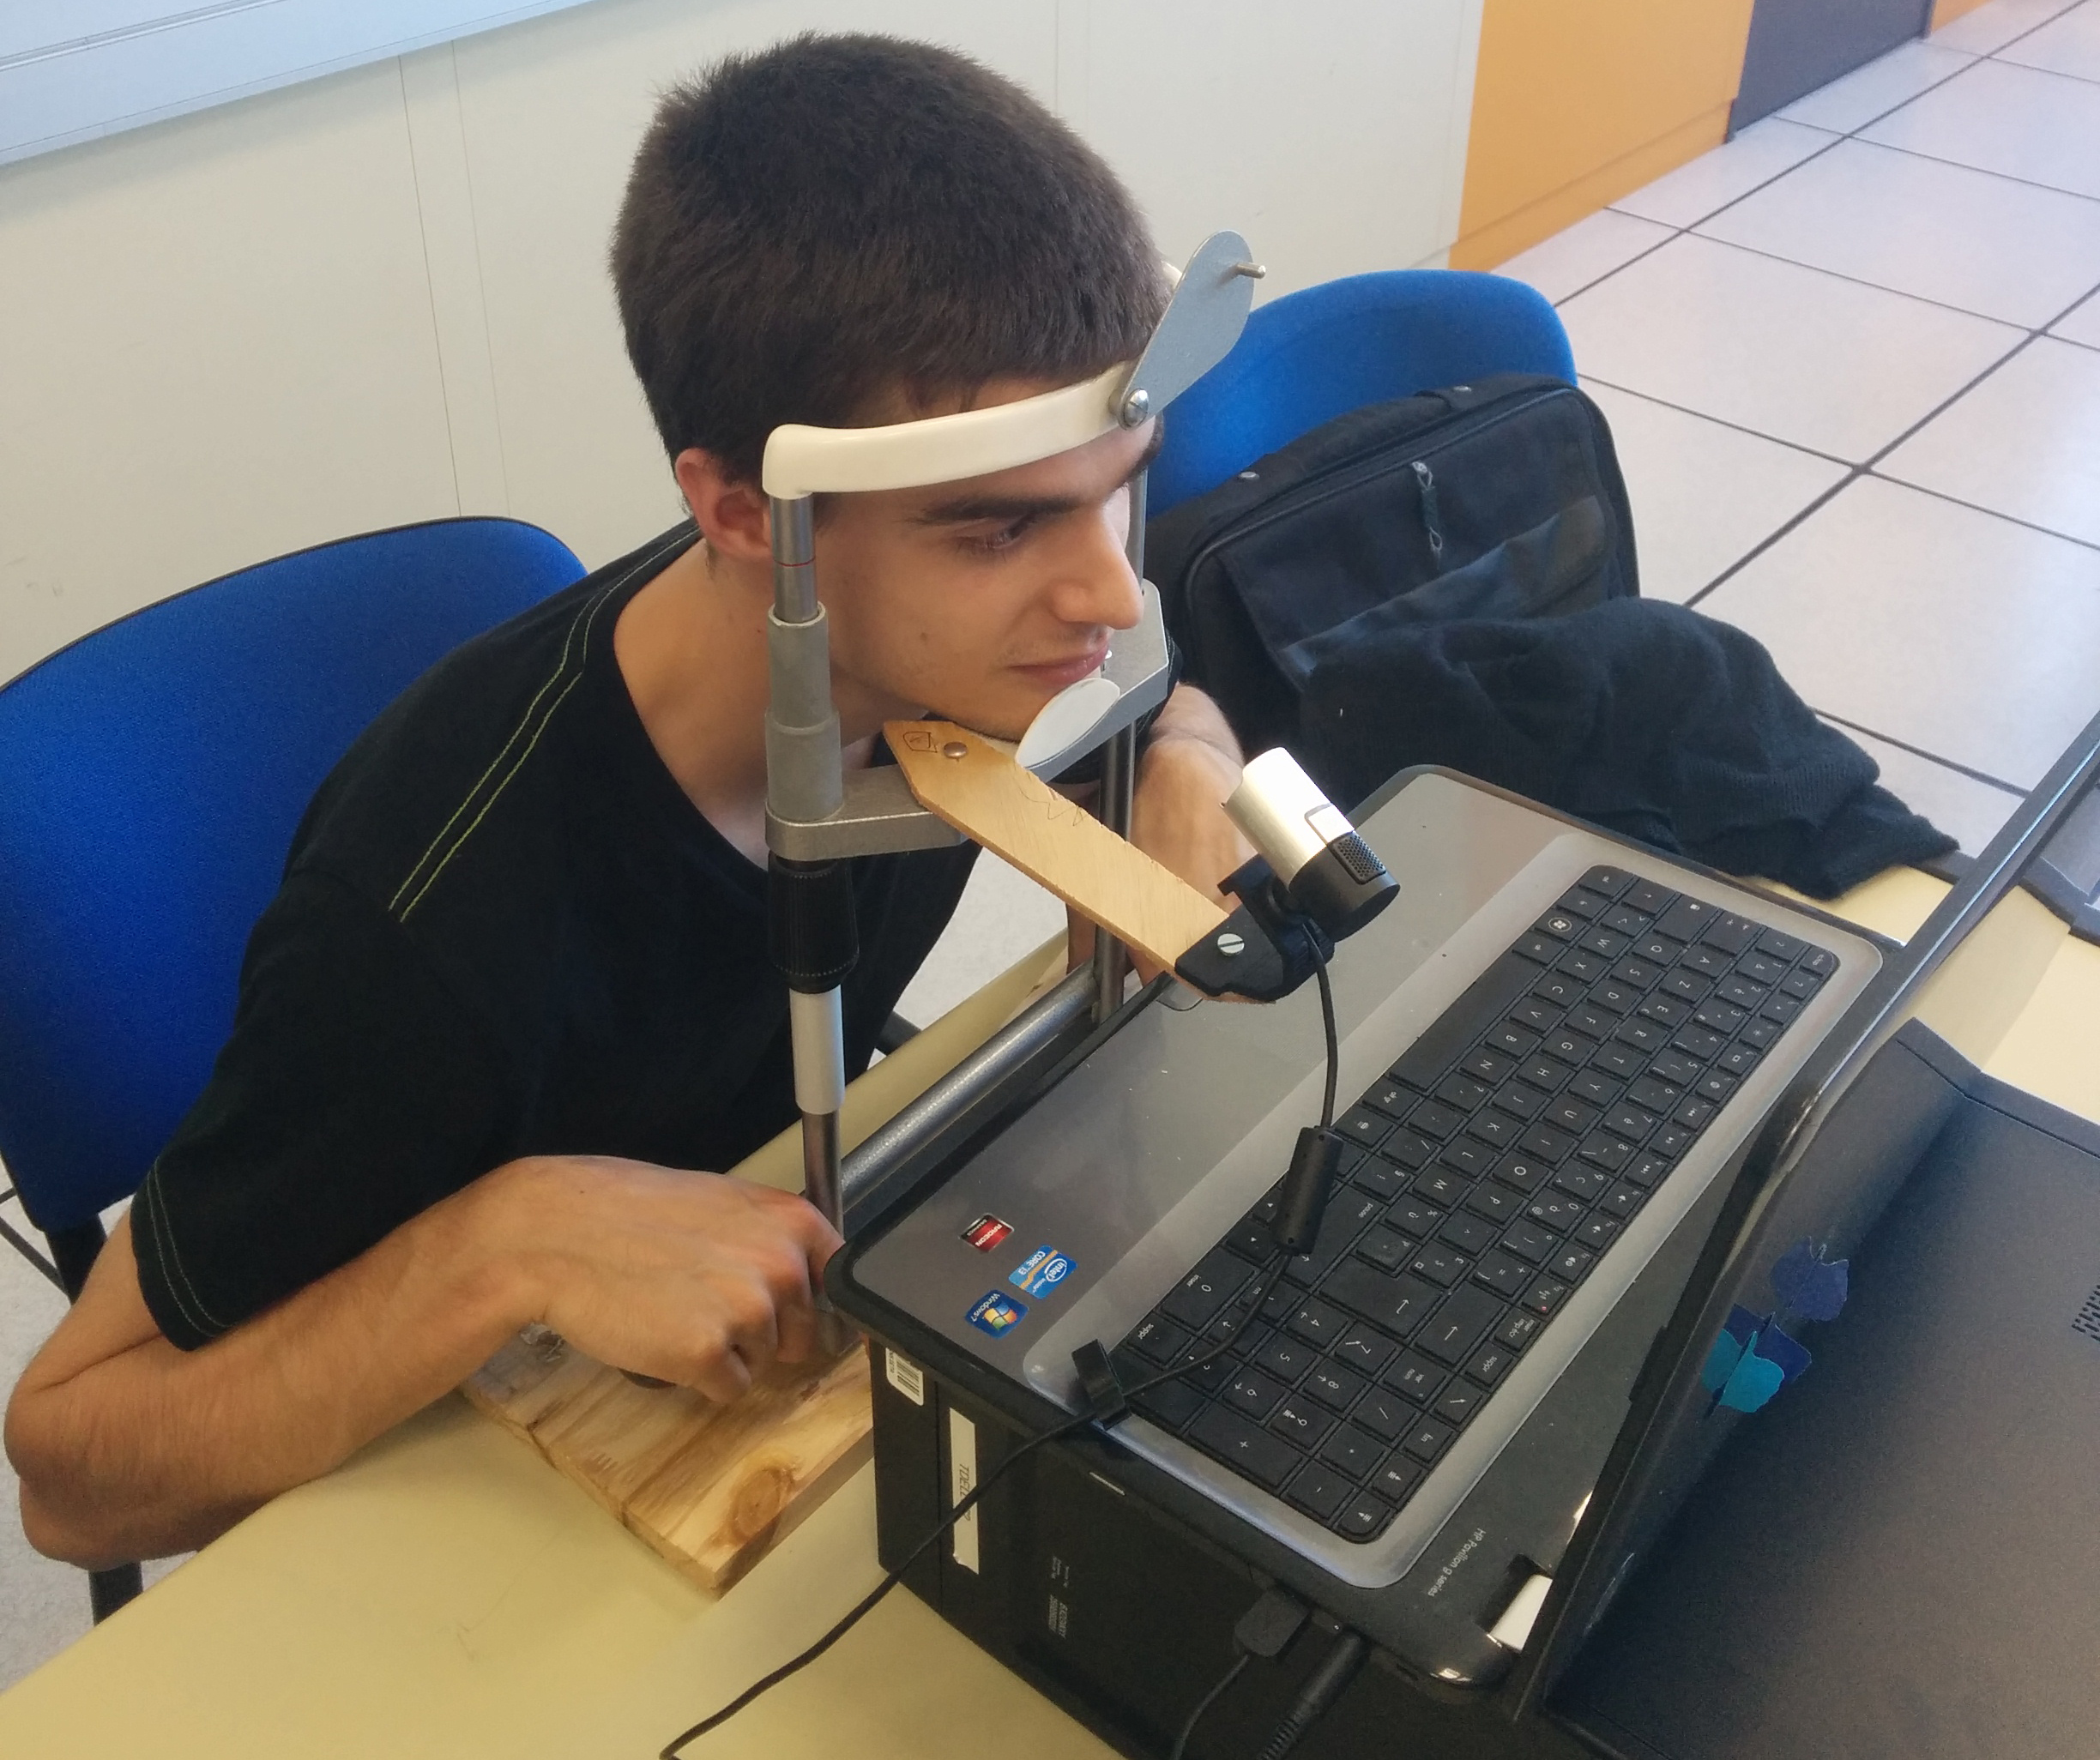
\includegraphics[scale=0.1]{Systeme}
  \caption{Interface d'acquisition composée de la caméra, fixée à la mentonnière}
  \label{fig:systeme}
\end{figure}

\subsection{Interface logicielle}
L'interface logicielle s'appuie sur le programme contenant des algorithmes développés en C++ avec OpenCV. Ils ont pour but de traiter les images transmises par la webcam afin de détecter le visage, puis les yeux et enfin les pupilles et les clignements pour déduire l'action que l'utilisateur souhaite effectuer. Que ce soit pour le clic ou le mouvement du curseur de la souris, une interaction avec l'OS est nécessaire. Le programme doit donc être adapté suivant le système d'exploitation utilisé.

\subsection{Interface graphique}
Enfin, le rôle de l'interface graphique (voir figure \ref{fig:IG9B2}) est de proposer à l'utilisateur un choix de boutons qui lancent des applications. Cette dernière est développée en C++ à l'aide de Qt Creator et ne peut être utilisée que sur Windows car il faudrait changer toutes les commandes d'ouverture d'applications pour exécuter le programme sur un autre système d'exploitation.

\begin{figure}[H]
  \centering
  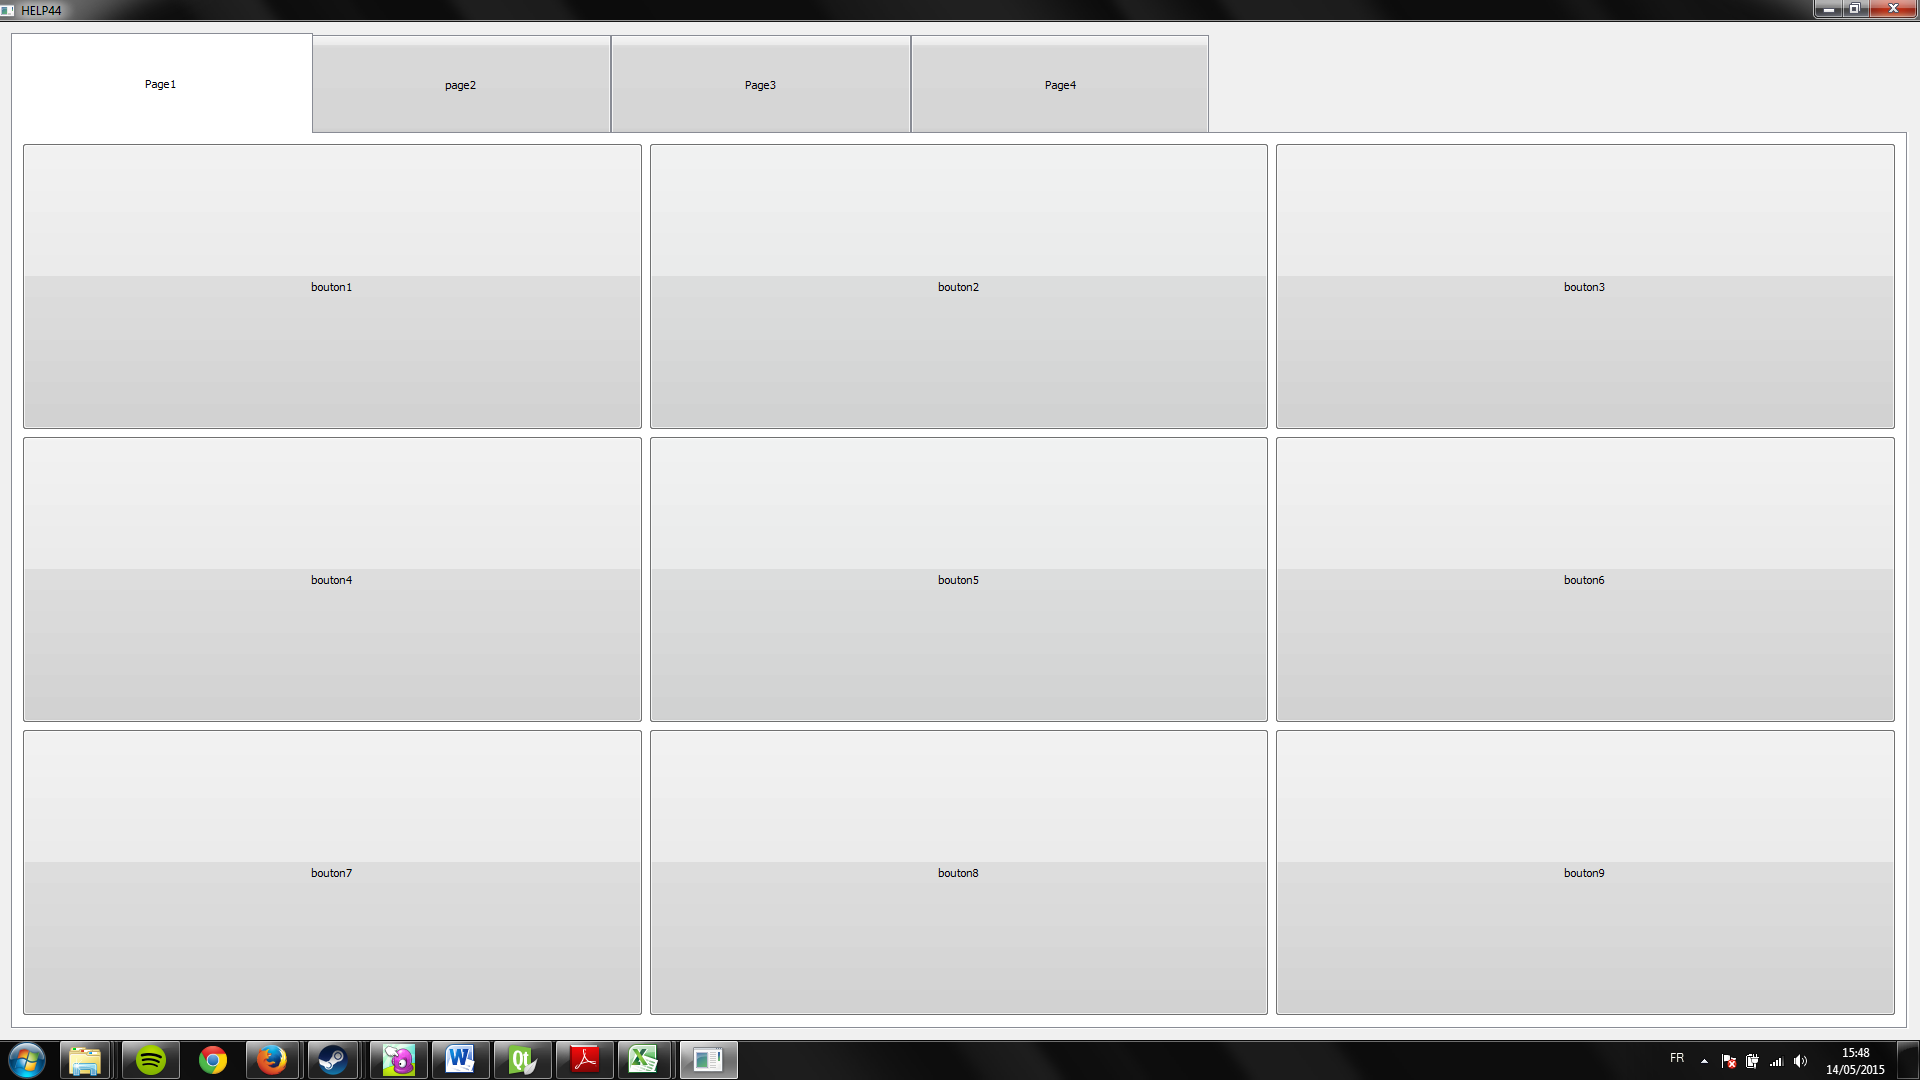
\includegraphics[scale=0.3]{IG9B}
  \caption{Interface graphique 9 boutons}
  \label{fig:IG9B2}
\end{figure}

\section{WBS}
La structure de découpage du projet découle de l'architecture physique. La figure \ref{fig:WBS} illustre le WBS ainsi établi. 

\begin{figure}[H]
  \centering
  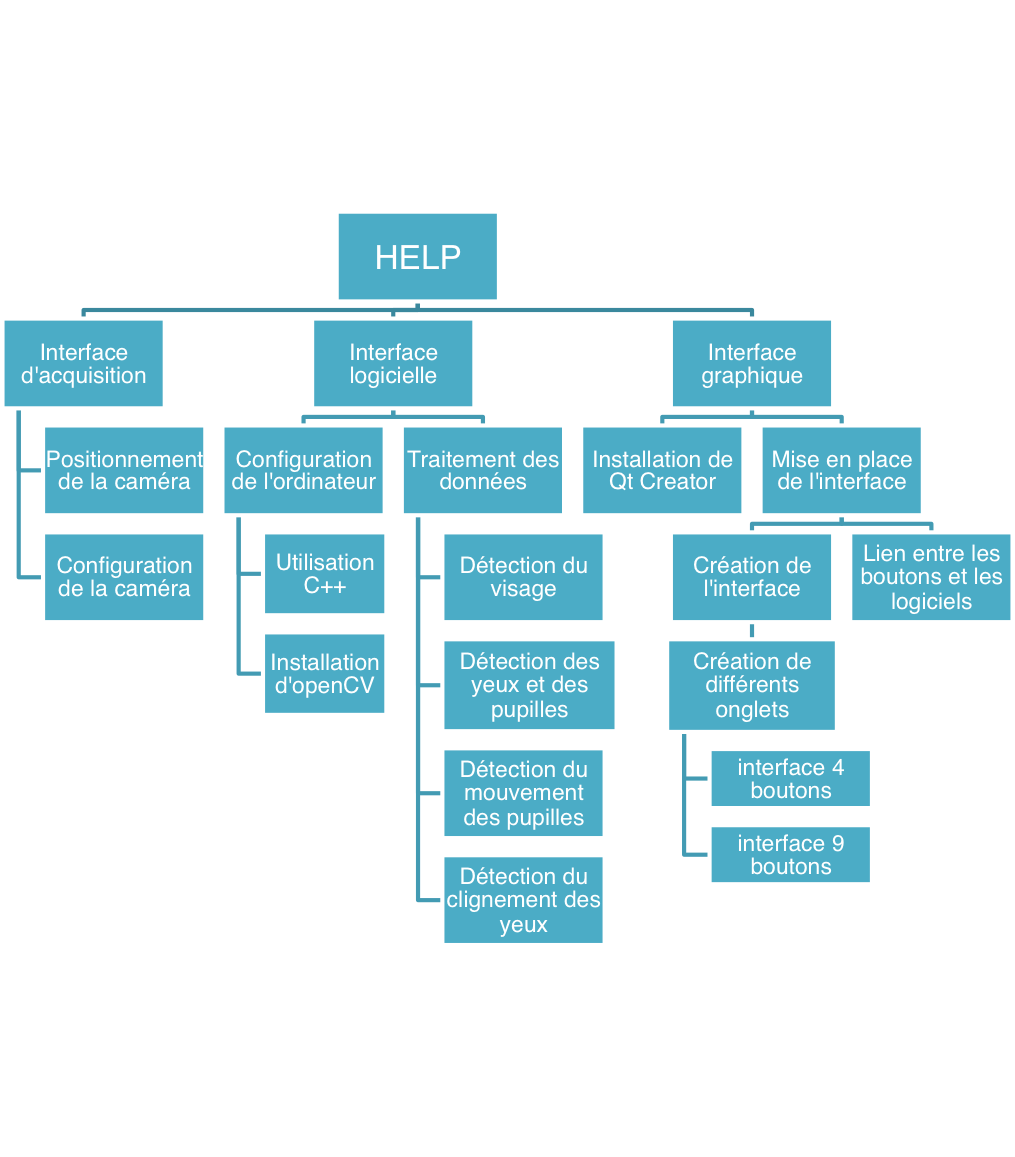
\includegraphics[scale=0.8]{WBS}
  \caption{WBS}
  \label{fig:WBS}
\end{figure}

\section{Matériel utilisé}

Comme présenté sur l'architecture physique, nous avions besoin de matériel pour réaliser notre système.

\subsection{Ordinateur}
L'ordinateur s'est naturellement imposé comme matériel nécessaire au projet, puisque l'utilisateur devait pouvoir utiliser quelques unes de ses fonctionnalités de base. De plus, pour traiter le flux d'images filmées, nous avions besoin d'une puissance de calcul suffisante. Ainsi, l'ordinateur a un double rôle. Il permet d'afficher l'interface graphique, et également d'obtenir l'action demandé par l'utilisateur, grâce à des algorithmes écrits en C++, s'appuiant sur OpenCV. 

\subsection{Caméra}
Si de nombreux types de caméras sont possibles, nous avons retenu la webcam. En effet, la résolution des webcams HD actuelles est largement suffisante pour une détection de pupilles. De plus, elles sont simples d'utilisation, car faciles à installer grâce au port usb d'un ordinateur. Il est aussi aisé de récupérer les flux vidéos. Nous pouvons également noter que les webcams sont relativement peu coûteuses.
Parmi celles-ci, nous avons sélectionné la LifeCam Studio HD 1080p (voir figure \ref{fig:Cam}), pour son bon rapport qualité prix. En effet, la grande résolution HD 1080p (1920x1080) permet un bon tracking des pupilles.

\begin{figure}[H]
  \centering
  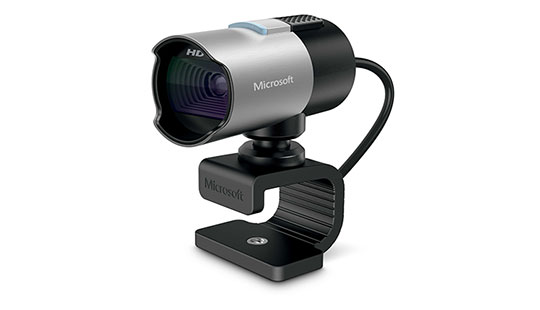
\includegraphics[scale=0.5]{cam}
  \caption{LifeCam Studio HD 1080p \\Source : Microsoft}
  \label{fig:Cam}
\end{figure}

\subsection{Mentonnière}

Afin que les coordonnées du centre des pupilles soient exploitables pour le suivi du regard, nous avions besoin que la tête reste fixe. En effet, lorsque la tête était libre de tout mouvement, les données collectées ne permettait pas de calibrer le programme. La solution de la mentonnière (figure \ref{fig:Menton}) a ainsi émergée. De plus, étant donné que le système vise à être utilisé par la suite par des personnes tétraplégiques, l'immobilisation de la tête ne soulève pas d'incohérence.
Enfin, nous avons fabriqué une planche de bois pour fixer dans un premier temps la caméra près de l'oeil. 

\begin{figure}[H]
  \centering
  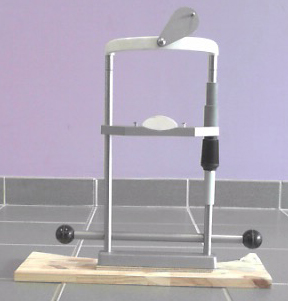
\includegraphics[scale=0.6]{Mentonniere}
  \caption{Mentonnière}
  \label{fig:Menton}
\end{figure}